\documentclass{ctexart} % 文档类对中英文混排支持较好
\usepackage{graphicx}
\usepackage{fancyhdr}
% \usepackage{DTMdate}
\usepackage[a4paper, left=2.5cm, right=2cm, top=2cm, bottom=2cm]{geometry}

% 设置摘要和关键字
\ctexset{
  abstractname = {\heiti \zihao{3} 摘\quad要},
}
% 设置章节和标题格式
\ctexset{
  section = {
    % 正确的写法:使用 'format' 键来设置标题的样式
    format = {\heiti \zihao{3} \raggedright},
  },
  subsection = {
    format = {\heiti \zihao{-3} \raggedright},
  },
  subsubsection = {
    % 注意:通常subsubsection的字号应该比subsection小
    % 如果 subsection 是 \zihao{-3} (小三),那么 subsubsection 应该是 \zihao{-4} (小四) 或更小
    format = {\heiti \zihao{-4} \raggedright}, % 已根据层级调整字号建议
  },
}
% 设置正文文本格式
\setmainfont{Times New Roman}
\setCJKmainfont{SimSun}
\AtBeginDocument{\zihao{-4}}



% 设置页眉页脚

\pagestyle{fancy}
\fancyhf{}
\fancyfoot[C]{\zihao{5}\thepage}

% 设置页眉
\fancyhead[R]{\zihao{-5} 数据结构实习}

\begin{document}
  \thispagestyle{empty} % 确保没有页眉页脚
  \vspace*{3.5cm}
  \begin{center}
    {\zihao{2}\ 信息工程学院}\\
    \vspace{1.5cm}
    {\zihao{1}\heiti 数据结构综合训练}\\
    \vspace{2cm}
    {\zihao{-4} (2024\~2025学年第二学期)}
  \end{center}
  \vspace{2cm}

  \begin{center}
    {\zihao{-3}\heiti 报告题目:\underline{简易神经网络的实现}} \\
    \vspace{4cm} % 
       \begin{tabular}{@{}p{3cm}p{8cm}@{}}
      {\zihao{-3}\heiti 姓名:} & {\zihao{-3}\heiti \underline{\makebox[8cm][c]{曾瑞安}}} \\
      {\zihao{-3}\heiti 专业:} & {\zihao{-3}\heiti \underline{\makebox[8cm][c]{计算机科学与技术}}} \\
      {\zihao{-3}\heiti 年级班级:} & {\zihao{-3}\heiti \underline{\makebox[8cm][c]{2023级计算机科学与技术2班}}} \\
      {\zihao{-3}\heiti 学号:} & {\zihao{-3}\heiti \underline{\makebox[8cm][c]{2023013332}}} \\
      {\zihao{-3}\heiti 指导教师:} & {\zihao{-3}\heiti \underline{\makebox[8cm][c]{耿耀君}}} \\
      {\zihao{-3}\heiti 完成日期:} & {\zihao{-3}\heiti \underline{{\makebox[8cm][c]{2025年07月16日}}}} \\
    \end{tabular}
  \end{center}
\clearpage

% 第一章
\section{综合训练目的和要求}
  本综合训练是计算机科学与技术、信息管理与信息系统、软件工程、电子商务专业重要的实践性环节之一,是在学生学习完《面向对象程序设计(C++)》、《数据结构》课程后进行的一次全面的综合练习。本课综合训练的目的和任务:\\
  1. 巩固和加深学生对C++语言、数据结构课程的基本知识的理解和掌握\\
  2. 掌握C++语言编程和程序调试的基本技能\\
  3. 利用C++语言进行基本的软件设计\\
  4. 掌握书写程序设计说明文档的能力\\
  5. 提高运用C++语言、数据结构解决实际问题的能力\\

\section{综合训练具体内容}

\subsection{神经网络核心框架设计与构建:}

\textbf{计算图的抽象化设计:} 项目的核心是将神经网络的运算流程抽象为一个有向无环图(DAG)。我们设计了 Node(节点)与 Graph(图)两个核心类。Node 封装了 Matrix(矩阵)作为其运算值,并存储了指向其父节点的 weak\_ptr,以此构建出完整的计算依赖关系。这种设计使得网络结构的定义极为灵活,能够动态地构建任意复杂度的网络模型。\\
\textbf{正向传播的实现:} 通过将加法、乘法、激励函数(如 Sigmoid)等操作均封装为建立新节点的函数 (ops),我们实现了直观的正向计算流程。每一步运算都会在计算图中产生一个新的 Node,并记录其与父节点的依赖关系,为后续的反向传播奠定基础。\\

\subsection{反向传播与拓扑排序的实现:}

\textbf{拓扑排序的应用:} 为了实现自动微分(Auto-differentiation),我们在 Node 的 backward() 方法中,首先对整个计算图进行拓扑排序。通过深度优先搜索(DFS)从损失节点开始遍历所有父节点,我们得到了一个反向的节点计算序列。这个序列确保了在计算任何节点的梯度之前,其所有后续节点的梯度都已经计算完毕,完美地解决了链式法则中的依赖问题。\\
\textbf{自动梯度计算:} 每个运算操作在建立 Node 的同时,都会通过 std::function 动态地为其绑定一个 \_backward 函数。在拓扑排序后的反向传播过程中,每个节点会依序执行自己的 \_backward 函数,将上游传来的梯度(存储在自身的 grad 矩阵中)根据该节点的运算类型(如加法、乘法)正确地传递给其父节点,从而实现了全自动的梯度计算与分发。\\

\subsection{模型训练与数据增强实践:}

利用构建好的框架搭建一个用于 MNIST 手写数字识别的 MLP 模型。在训练过程中,为了提升模型的泛化能力以适应真实、多样的手写笔迹,我们引入了数据增强技术。在每个训练批次中,对输入的 28x28 图像矩阵进行随机的空间变换(平移、旋转)与像素级干扰(高斯噪声),极大地丰富了训练样本,使模型学习到更鲁棒的数字特征。\\

\subsection{端到端系统集成与部署:}

将训练好的模型参数存储,并在一个基于 Qt 的图形化桌面应用中进行集成。应用程序内部实现了一套完整的图像预处理管线,能将用户在画布上书写的任意笔迹,标准化为与训练时一致的 28x28 矩阵格式。最终,应用程序直接在内部调用神经网络框架执行预测,并实时反馈识别结果,完成了从底层算法到上层应用的完整技术闭环,验证了整个框架的实用性与正确性。\\

\section{总体设计}
\subsection{项目组成}
本项目框架主要可分为\textbf{核心类}、\textbf{核心计算}、\textbf{模型训练}、\textbf{前端展示}.
\subsubsection{核心类}
在core 中我们设计了Matrix作为矩阵管理类,并封装相应的计算函数,在设计时我们使用一维数组来模拟二维数组,在内存读取方面更容易命中,增加计算的速度.\\
我们设计了Node类作为图的节点类,每个节点内部含有两个Matrix类,分别作为前向计算值和反向计算梯度,并使用vector<weak<>>方式持有自己的父节点.\\
设计Graph类作为Node友元类,并删除Node创造函数确保所有的Node节点都由Graph管理,便于内存管理.
\subsubsection{核心计算}
核心计算代码位于src/opts文件夹中\\
我们设计了ops文件包含所有函数计算,对于每个运算我们都会创建一个新的Node节点并设置对应的反向传播函数,并确保由Graph管理.\\
\subsubsection{模型训练}
为了验证模型的可行性,我们设计完成手写数字识别,并将其作为我们的展示,我们使用一个输入层、一个隐藏层、以及一个输出层,由于我们设计的模型是动态生成节点因此在后续添加隐藏层较为容易,亲自测试每天加一个隐藏层不超过5行代码.\\
为了读取文件我们设计了DataLoader与DataSet作为基类并封装了相应的方法,并设计了CsvDataLoader作为本次手写数字识别的读取类.
\subsubsection{前端展示}
基于QT的图形化界面应用,并能够让用户书写任何内容,通关按钮将画布内容转为28*28矩阵并输出对应预测结果.

\subsection{框图与流程图}
\subsubsection{程序组成框图}
\begin{figure}[htbp]
  \centering
  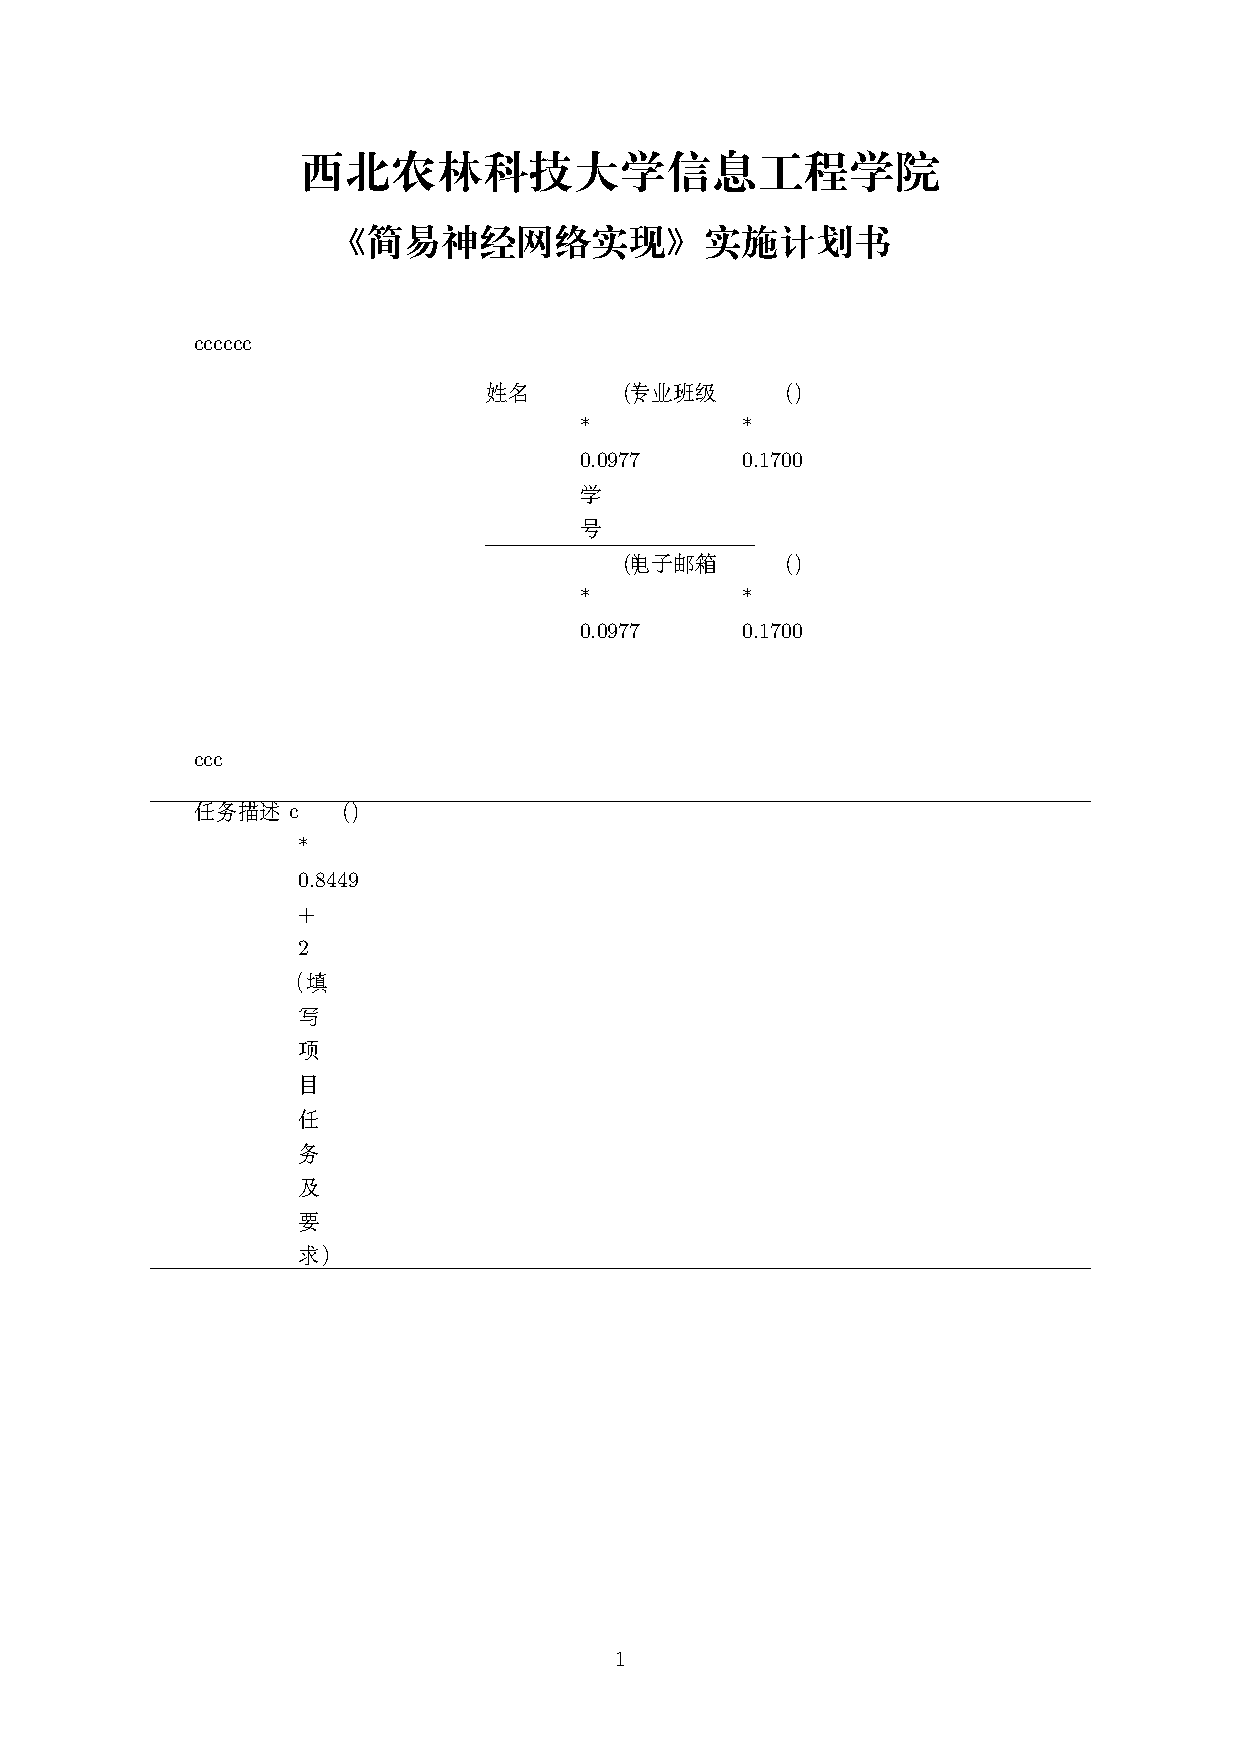
\includegraphics[width=0.7\textwidth]{./1.png}
  \caption{框图}
  \label{fig:my_awesome_figure}
\end{figure}
\subsubsection{流程图}
\begin{figure}[htbp]
    \centering
    % 第一个图的 minipage
    \begin{minipage}[t]{0.48\textwidth} % [t]表示顶部对齐,0.48\textwidth表示占用当前文本宽度48%
        \centering
        \includegraphics[width=1\linewidth]{./2.png} % width=1\linewidth表示图片宽度占满minipgae的宽度
        \caption{模型训练流程图}
        \label{fig:model_training} % 建议添加标签以便引用
    \end{minipage}
    \hfill % 填充空白,使两个 minipage 之间有弹性间距
    % 第二个图的 minipage
    \begin{minipage}[t]{0.48\textwidth}
        \centering
        \includegraphics[width=1\linewidth]{./3.png}
        \caption{手写数字识别}
        \label{fig:handwriting_recognition} % 建议添加标签以便引用
    \end{minipage}
    % 注意:整个figure环境只需要一个 \caption 和 \label,
    % 如果每个图都有独立小标题,则如上面所示,每个minipage里一个caption
    % 如果只需要一个总标题,则把两个minipage里的caption移到figure环境的底部
    % \caption{模型训练流程图与手写数字识别} % 如果只有一个总标题,则用这个
    % \label{fig:two_figures}
\end{figure}

\section{详细设计说明}
整体代码分为四个模块,{核心类模块}
\end{document}
